%%% This example illustrates the basic elements of a progress report
%%%
\documentclass[a4paper,11pt]{article}
	\usepackage{a4wide}
	\usepackage [final] {graphicx} % graphics package
	\usepackage{psfrag}  % figure text formatting package
	\usepackage{xcolor}  % graphics package
	\usepackage{amssymb} % mathematical symbol package
	\usepackage{amsmath} % mathematical symbol package
	
	\pagestyle{myheadings}
	
	%%%%%%%%%%%%%%%%%%%%%%%%%%%%%%%%%%%%%%%%%%%%%%%
	%%% You should edit this part appropriately
	\newcommand{\Title}{Progress Report A. de Windt}
	\newcommand{\Author}{A. de Windt}
	\newcommand{\Date}{21-01-2019}
	\newcommand{\Subject}{Policy Gradient Reinforcement Learning for quadrotor control}
	\newcommand{\Mentors}{Dr.ir. Erik-Jan van Kampen}
	
	\newcommand{\Term}{09/2018 - 07/2019}
	\newcommand{\Mail}{A.deWindt@student.tudelft.nl}
	%%%%%%%%%%%%%%%%%%%%%%%%%%%%%%%%%%%%%%%%%%%%%%%
	
	\begin{document}
	%%%%%%%%%%%%%%%%%%%%%%%%%%%%%%%%%%%%%%%%%%%%%%%
	\markright{\footnotesize\textnormal{\textbf{\Title}}~~~\Author}
	\thispagestyle{plain} \noindent
	Delft University of Technology\\
	Department of Control \& Simulation\\
	\par\begin{center}
	{\LARGE\textbf{\Title}}\par\bigskip{\large \Author}
	\end{center}
	\par\bigskip
	\begin{center}{\small
	\begin{tabular}{ll}\hline
	\textbf{Date:}& \Date\\
	\textbf{Subject:}& \Subject\\
	\textbf{Supervisors:}& \Mentors\\
	\textbf{Project term:} & \Term\\
	\textbf{E-mail:} & \Mail\\\hline
	\end{tabular}}
	\end{center}
	\par\bigskip
	%%%  End Header
	%%%%%%%%%%%%%%%%%%%%%%%%%%%%%%%%%%%%%%%%%%%%%%%
	
	
	\section*{Outcome of the previous meeting}
	
	\begin{itemize}
		\item Didn't do much progress.
	\end{itemize}
	
	\section*{Description of the results since last meeting}

	\subsection*{Short version}
	\begin{itemize}
		\item Asside from reading a few papers, I didn't do much progress.
	\end{itemize}
	
	\section*{Plans for next 2 weeks}
	% Same as last week, since I havn't been able to progress.
	\begin{enumerate}
	\item Finish inverted pendulum example.
	\item Try out modifications to the example. (Use Neural Network, etc)
	\item Read through literature again and filter out the most relevant and summize them. 
	\item Start writing report. (Explain RL examples, literature summaries)
	\end{enumerate}
	
	
	
	\begin{appendix}
	% 	\section{Simulation results}
	% \begin{figure}[h]
	% 	\caption{Sum of rewards at each episode.}
	% 	\centering
	% 	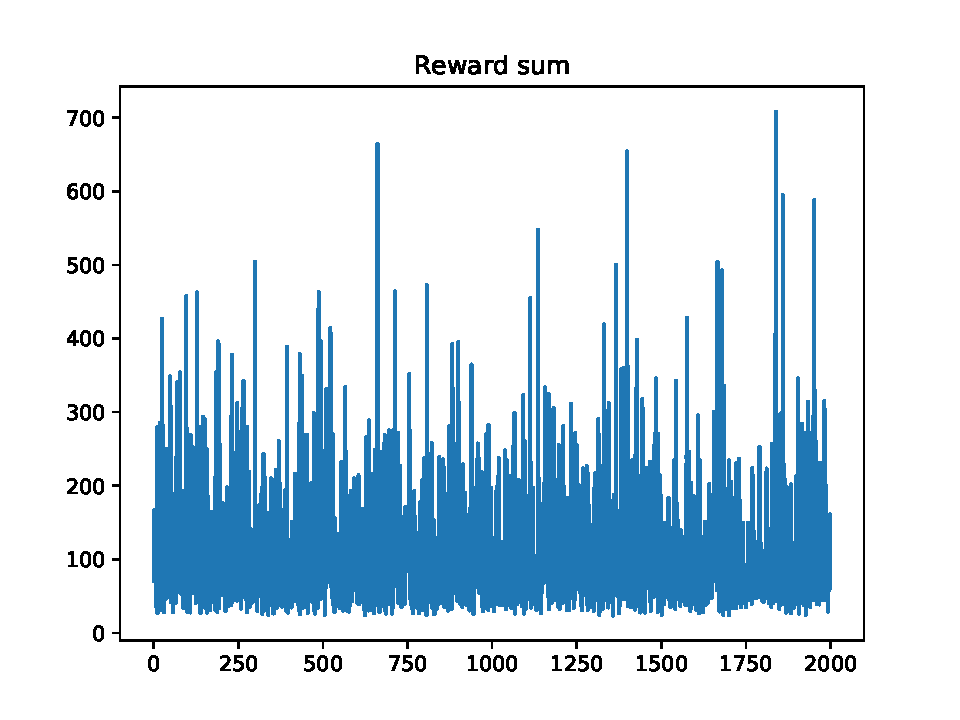
\includegraphics[width=0.9\textwidth]{figures/r_sum}
	% \end{figure}

	% \begin{figure}[h]
	% 	\caption{First episode.}
	% 	\centering
	% 	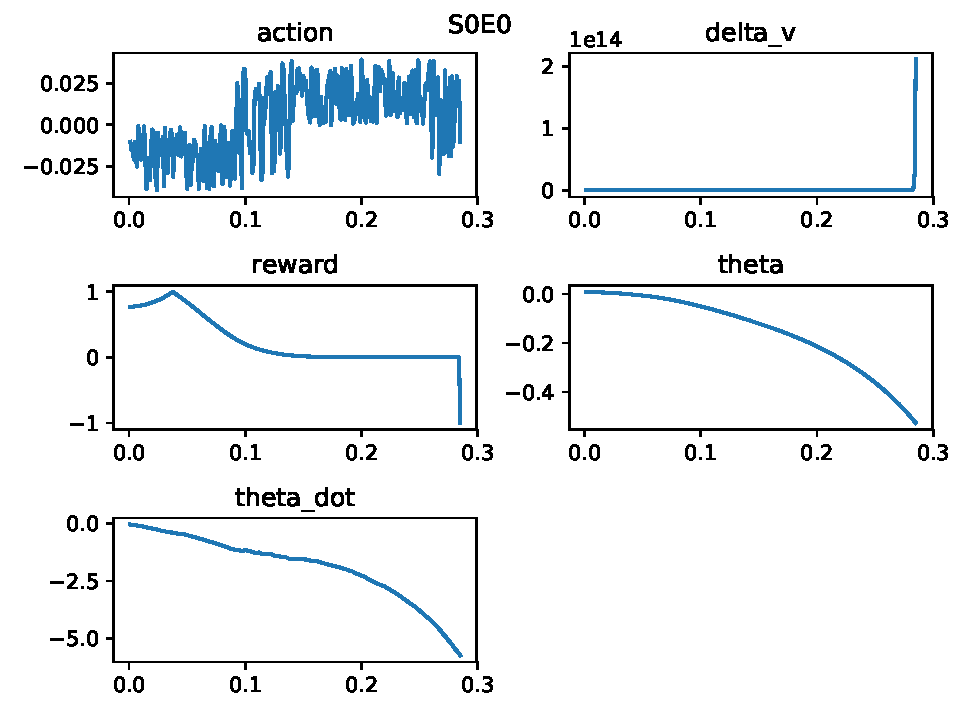
\includegraphics[width=0.9\textwidth]{figures/first_episode}
	% \end{figure}
	
	% \begin{figure}[h]
	% 	\caption{Last episode.}
	% 	\centering
	% 	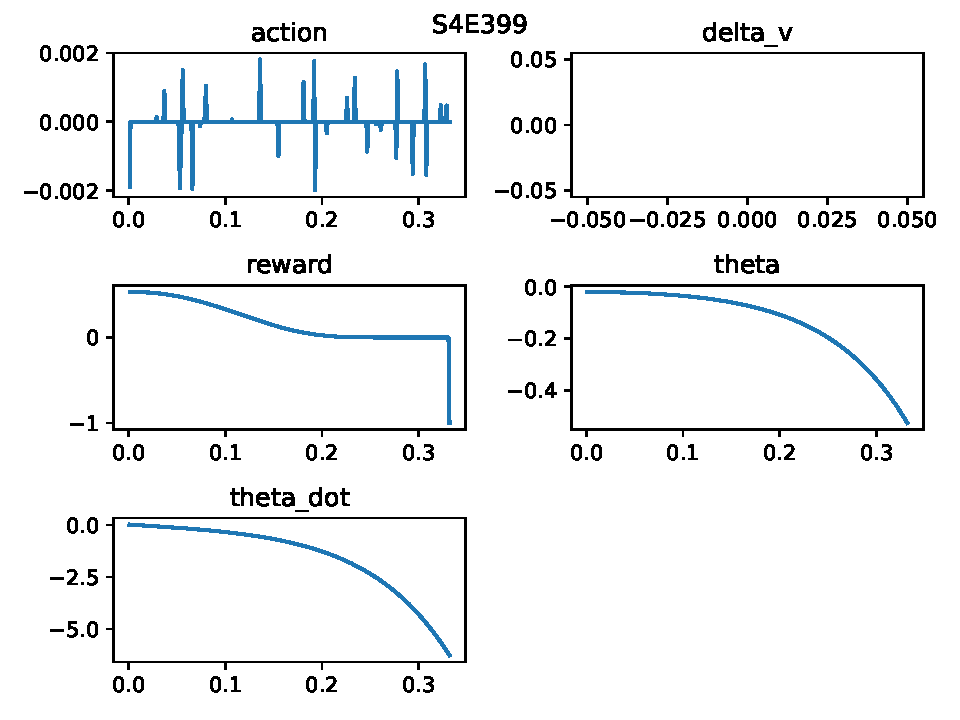
\includegraphics[width=0.9\textwidth]{figures/last_episode}
	% \end{figure}

	\end{appendix}


	% \section{An example appendix}
	% Here is an example of an inline equation: $a^2 = b^2 + c^2$. 
	
	% Here is an example of a display equation:
	% \begin{equation}
	% 	\mathbf{S} = \mathbf{G}^{-1} \mathbf{x} + n
	% 	%B_{\kappa}^d(\mathbf{b}) := \frac{d!}{\kappa!}\mathbf{b}^{\kappa} ,
	% \label{eq:sensormodel}
	% \end{equation}
	
	% You can refer to the display equation using the label: Eq \ref{eq:sensormodel} references the above equation. Note that you have to rebuild the documents 3 times to update references. You can also refer to figures, as follows: Fig \ref{fig:splineWFR_costfnnorms} refers to the figure in the other appendix.
	
	
	% \section{An example figure}
	
	% In this appendix an eps figure is printed. The figure was made in Matlab, and text captions are contained in the fig\_SplineFD\_NormComp\_G10.tex file. 
	
	% \begin{figure}
	% 	 \centering
	% 	 \begin{psfrags}%
	% 	 \psfragscanon%
	% 	 % Generated using matlabfrag
% Version: v0.6.13
% Version Date: 11-Jan-2010
% Author: Zebb Prime
%
%% <text>
%
\providecommand\matlabtextA{\color[rgb]{0.000,0.000,0.000}\fontsize{10}{10}\selectfont\strut}%
\psfrag{015}[cl][cl]{\matlabtextA FD $\sigma^2||L||_2^2$}%
\psfrag{016}[cl][cl]{\matlabtextA FD $||I-LD||_2^2$}%
\psfrag{017}[cl][cl]{\matlabtextA Spline $\sigma^2||L||_2^2$}%
\psfrag{018}[cl][cl]{\matlabtextA Spline $||I-LD||_2^2$}%
\psfrag{019}[bc][bc]{\matlabtextA Comparison of FD and Spline Cost Function Partial Norms on 10x10 grid}%
\psfrag{020}[bc][bc]{\matlabtextA Norms}%
\psfrag{021}[tc][tc]{\matlabtextA $Sigma^2$}%
%
%% </text>
%
%% <xtick>
%
\def\matlabfragNegXTick{\mathord{\makebox[0pt][r]{$-$}}}
%
\psfrag{000}[ct][ct]{\matlabtextA $10^{-10}$}%
\psfrag{001}[ct][ct]{\matlabtextA $10^{-8}$}%
\psfrag{002}[ct][ct]{\matlabtextA $10^{-6}$}%
\psfrag{003}[ct][ct]{\matlabtextA $10^{-4}$}%
\psfrag{004}[ct][ct]{\matlabtextA $10^{-2}$}%
\psfrag{005}[ct][ct]{\matlabtextA $10^{0}$}%
%
%% </xtick>
%
%% <ytick>
%
\psfrag{006}[rc][rc]{\matlabtextA $10^{-14}$}%
\psfrag{007}[rc][rc]{\matlabtextA $10^{-12}$}%
\psfrag{008}[rc][rc]{\matlabtextA $10^{-10}$}%
\psfrag{009}[rc][rc]{\matlabtextA $10^{-8}$}%
\psfrag{010}[rc][rc]{\matlabtextA $10^{-6}$}%
\psfrag{011}[rc][rc]{\matlabtextA $10^{-4}$}%
\psfrag{012}[rc][rc]{\matlabtextA $10^{-2}$}%
\psfrag{013}[rc][rc]{\matlabtextA $10^{0}$}%
\psfrag{014}[rc][rc]{\matlabtextA $10^{2}$}%
%
%% </ytick>
	% 	 \resizebox{10cm}{!}{
\includegraphics{figures/fig_SplineFD_NormComp_G10.eps}}%
	%  %\includegraphics{figures/fig_CuRe_WavefrontXY_G21x21_NL15_NR1.eps}
	% 	 \end{psfrags}
	% 	 \caption{Linear estimator cost function partial norms for the Finite Difference and the Spline method.}
	% 	 \label{fig:splineWFR_costfnnorms}
	% \end{figure}
	
	
	% \end{appendix}
	
	
	\end{document}
	